\documentclass[border=10pt]{standalone}
\usepackage[svgnames]{xcolor}
\usepackage{amsmath}
\usepackage{pgfplots}
\pgfplotsset{compat=newest}
\usepackage[sfdefault]{FiraSans}
\usepackage{FiraMono}
\renewcommand*\familydefault{\sfdefault}
\begin{document}
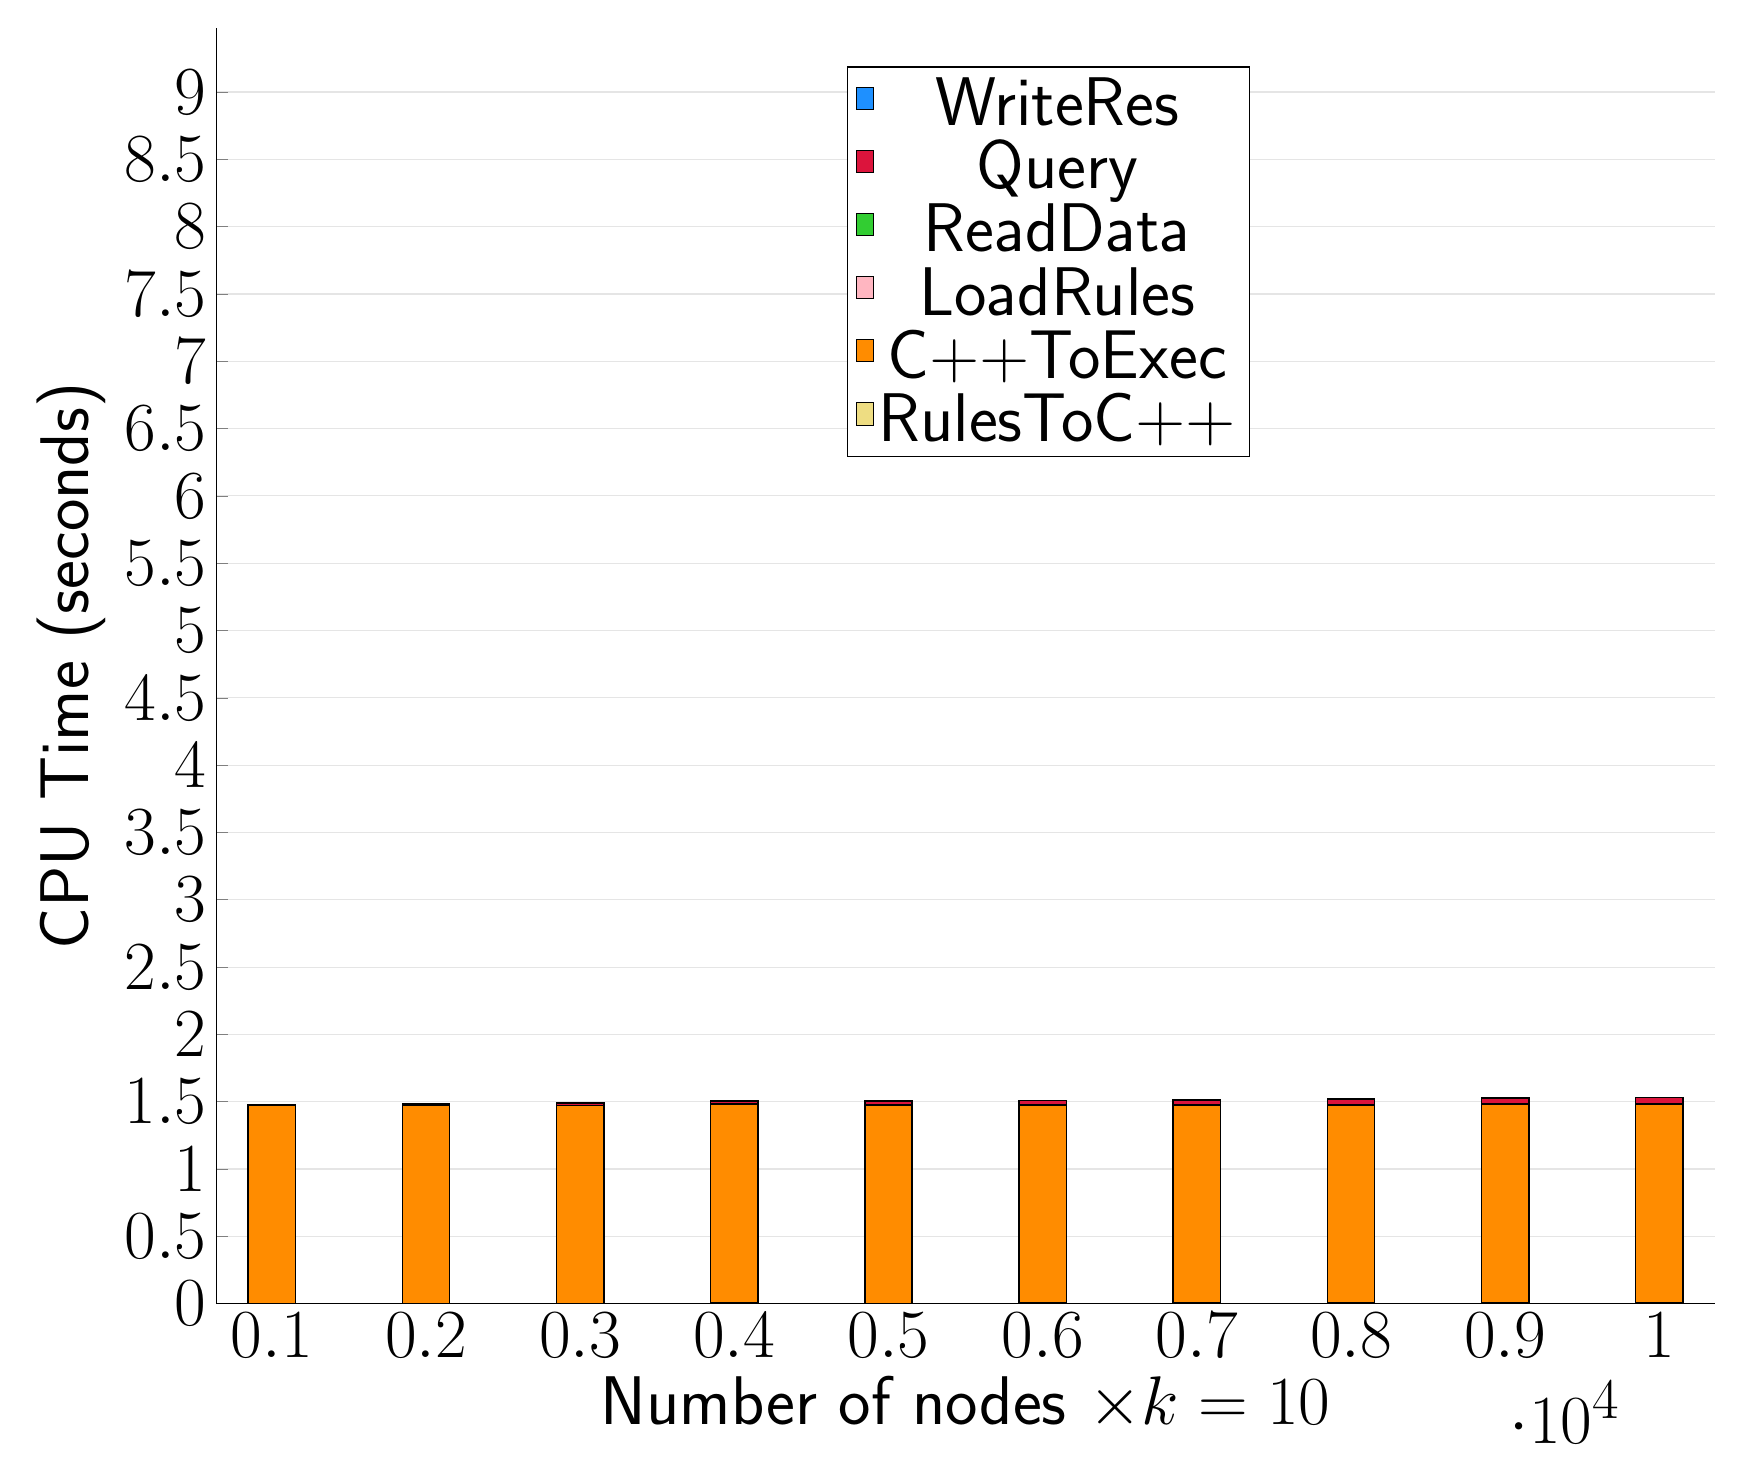
\begin{tikzpicture}
\begin{axis}[
   ybar stacked,
   width=1.7\textwidth,
   bar width=0.6cm,
   ymajorgrids, tick align=inside,
   major grid style={draw=gray!20},
   xtick=data,
   ymin=0, ymax=9.474,
   axis x line*=bottom,
   axis y line*=left,
   enlarge x limits=0.04,
   legend style={
       at={(0.69, 0.97)},
       anchor=north east,
       legend columns=1,
       font=\Huge,
   },
   ylabel={CPU Time (seconds)},
   xlabel={Number of nodes $\times k=10$},
   label style={font=\Huge},
   tick label style={font=\Huge},
]
\addlegendimage{fill=DodgerBlue, draw=black, line width=0.2pt}
\addlegendentry{WriteRes}
\addlegendimage{fill=Crimson, draw=black, line width=0.2pt}
\addlegendentry{Query}
\addlegendimage{fill=LimeGreen, draw=black, line width=0.2pt}
\addlegendentry{ReadData}
\addlegendimage{fill=LightPink, draw=black, line width=0.2pt}
\addlegendentry{LoadRules}
\addlegendimage{fill=DarkOrange, draw=black, line width=0.2pt}
\addlegendentry{C++ToExec}
\addlegendimage{fill=LightGoldenrod, draw=black, line width=0.2pt}
\addlegendentry{RulesToC++}
\addplot +[fill=LightGoldenrod, draw=black, line width=0.55pt] coordinates {
(1000, 0.0)
(2000, 0.0)
(3000, 0.0)
(4000, 0.008000000000000002)
(5000, 0.0020000000000000005)
(6000, 0.006000000000000001)
(7000, 0.004000000000000001)
(8000, 0.006000000000000001)
(9000, 0.008000000000000002)
(10000, 0.008000000000000002)
};
\addplot +[fill=DarkOrange, draw=black, line width=0.55pt] coordinates {
(1000, 1.47)
(2000, 1.4739999999999998)
(3000, 1.47)
(4000, 1.4739999999999998)
(5000, 1.472)
(6000, 1.468)
(7000, 1.47)
(8000, 1.47)
(9000, 1.472)
(10000, 1.4739999999999998)
};
\addplot +[fill=LightPink, draw=black, line width=0.55pt] coordinates {
(1000, 0.00018600000000000002)
(2000, 0.000201)
(3000, 0.0001866)
(4000, 0.0001784)
(5000, 0.000202)
(6000, 0.0001804)
(7000, 0.00018300000000000003)
(8000, 0.0001886)
(9000, 0.0001922)
(10000, 0.000177)
};
\addplot +[fill=LimeGreen, draw=black, line width=0.55pt] coordinates {
(1000, 0.0009090000000000001)
(2000, 0.001166)
(3000, 0.0016622000000000002)
(4000, 0.0019968)
(5000, 0.0024257999999999997)
(6000, 0.0027313999999999997)
(7000, 0.0030868)
(8000, 0.003209)
(9000, 0.0035226)
(10000, 0.004226199999999999)
};
\addplot +[fill=Crimson, draw=black, line width=0.55pt] coordinates {
(1000, 0.0072331999999999995)
(2000, 0.0113456)
(3000, 0.017309400000000003)
(4000, 0.021942200000000002)
(5000, 0.026856)
(6000, 0.0306346)
(7000, 0.0340246)
(8000, 0.036439)
(9000, 0.040304)
(10000, 0.0434414)
};
\addplot +[fill=DodgerBlue, draw=black, line width=0.55pt] coordinates {
(1000, 0.001042)
(2000, 0.0013376)
(3000, 0.001634)
(4000, 0.0018273999999999999)
(5000, 0.0020096)
(6000, 0.0022714)
(7000, 0.0024874)
(8000, 0.0026444000000000003)
(9000, 0.0027243999999999997)
(10000, 0.0029944000000000004)
};
\end{axis}
\end{tikzpicture}

\end{document}
